\newpage
\drawBar{Introductie - Vervolg}
\vspace*{0.2cm}
\deelhoofdstuk{Basis zetten}
\noindent
\begin{minipage}[t]{.48\textwidth}
  \zetKortKort{Hoger opleggen}{0.40}{1}{Een kaart op een \ul{lagere} kaart van \ul{hetzelfde} symbool leggen.}
  \zetKort{\'E\'entje lager opleggen en zelf drinken}{0.40}{2}{Een kaart op een kaart \\\ul{\'e\'en} hoger van \ul{hetzelfde} symbool leggen}{Proost op \quotes{offer Frits} en \textbf{neem een Fritsje}.}
\end{minipage}% This must go next to `\end{minipage}`
\hfill \vrule \hfill
\begin{minipage}[t]{.48\textwidth}
\vspace{-0.155cm}
  \zetKortKort{De aas en de 2}{0.40}{3}{Een \kaart{2} op een \kaart{aas} van \newline \ul{hetzelfde} symbool leggen.}
  \zetKortKort{De veelzijdige 9}{0.40}{4}{Een \kaart{9} op een kaart ongelijk aan een \kaart{joker} leggen.}
\end{minipage}


\deelhoofdstuk{Zetten - Laat andere spelers drinken}
\label{sec:regels_kort}

\zetLangKleinNew{ace_of_hearts}{king_of_diamonds}{king_of_spades}{ace_of_hearts}{Een \kaart{koning} op een \kaart{harten aas} leggen of andersom}{Andere spelers proosten op \quotes{kut Lisa} en \textbf{Fritsen}.}{}

\zetLangKleinNew{jack_of_clubs}{queen_of_hearts}{queen_of_diamonds}{jack_of_clubs}{Een \kaart{rode vrouw} op een \kaart{klaveren boer} leggen of andersom}{Andere spelers proosten op \quotes{Chantal} en \textbf{Fritsen}.}{}

\zetLangKleinNew{queen_of_diamonds}{queen_of_clubs}{queen_of_spades}{queen_of_hearts}{Een \kaart{vrouw} op een \kaart{vrouw} leggen}{Andere spelers proosten op \quotes{kut Kim} en \textbf{Fritsen}.}{\ul{\texttt{LET OP}}: Als de \kaart{vrouw} op een stapel met daarop al tenminste drie achtereenvolgende \kaart{vrouwen} wordt gelegd, moeten de andere spelers \textbf{een dubbele Frits nemen}.}{}

\zetLangKleinNew{9_of_clubs}{9_of_diamonds}{9_of_hearts}{9_of_spades}{Een \kaart{9} op een \kaart{9} leggen}{Andere spelers proosten op \quotes{iedereen dubbel Frits} en \textbf{nemen een dubbele Frits}.}{}

\zetLangKleinNewTweePunten{red_joker}{black_joker}{10_of_spades}{black_joker}{Een \kaart{joker} op de jokerstapel leggen}{Begin een nieuwe jokerstapel als er nog geen jokerstapel ligt.}{Andere spelers proosten op \quotes{Frits} en \textbf{Fritsen}.}{\ul{\texttt{LET OP}}: Er is maar \ul{\'e\'en} jokerstapel!\\ \ul{\texttt{LET OP}}: Niet uitgaan met deze zet!}

\vspace{0.525cm}

\centerline{\Large{\textbf{De volgende pagina bevat zetten voor ervaren spelers}}}

\newpage
\drawBar{Introductie - Vervolg}
\deelhoofdstukMetLabel{Zet - De koning en ass tegelijkertijd \proLabel}
\noindent
\vspace{-0.8cm}

\zetLangNewKoningAas{diamonds}{hearts}{spades}{clubs}{Een \kaart{koning} en een \kaart{aas} van hetzelfde symbool achterelkaar op een \kaart{vrouw} van hetzelfde symbool leggen}

\vspace{-1.0cm}
\deelhoofdstukMetLabel{Zet - Wissel je kaarten in \proLabel}
\noindent
\label{zetkort:thierry}
\vspace{-0.8cm}

\zetLangNewTweePunten{queen_of_diamonds}{6_of_hearts}{queen_of_clubs}{6_of_diamonds}{Een \kaart{6} op een \kaart{vrouw} leggen}{Leg je kaarten \ul{dicht} op de snijplank, proost op \quotes{Baudet} en \textbf{neem een dubbele Frits}.}{\Frits legt de kaarten onderop de dichte stapel en geeft je evenveel nieuwe kaarten.}{\ul{\texttt{LET OP}}: Niet uitgaan met deze zet!}

\vspace{-1.0cm}
\deelhoofdstukMetLabel{Zet - Blokkeer andere spelers \proLabel}
\noindent
\label{zetkort:caroline}
\vspace{-0.8cm}

\zetLangNewTweePunten{6_of_clubs}{jack_of_diamonds}{6_of_hearts}{jack_of_spades}{Een \kaart{boer} op een \kaart{6} leggen}{Plaats een shotglaasje op \'e\'en van de open stapels, proost op \\ \quotes{van der Plas} en \textbf{neem een dubbele Frits}.}{Niemand mag nu opleggen op de stapel met het shotglaasje en die er orthogonaal aan grenzen.}{\ul{\texttt{LET OP}}: Haal het shotglaasje in volgende beurt als eerste weer weg! \\ \ul{\texttt{LET OP}}: Niet uitgaan met deze zet!}

\vspace{0.25cm}

\noindent
\begin{minipage}[t]{.48\textwidth}
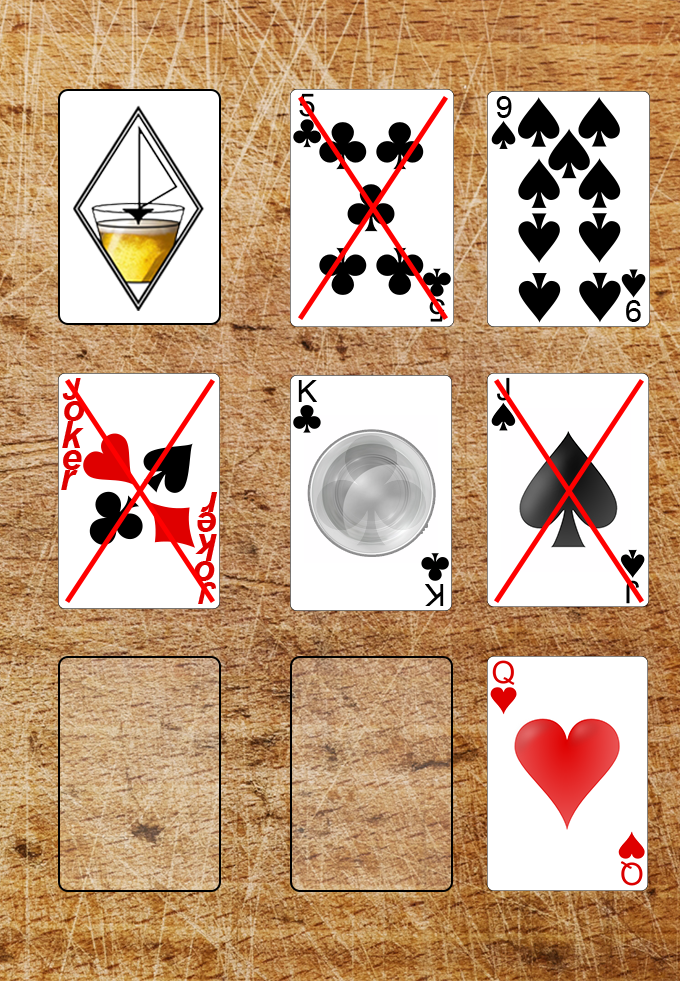
\includegraphics[width=.96\textwidth]{img/cards/Frits_plank_Carolinetje.png}
\end{minipage}
\hfill \vrule \hspace{0.35cm}
\begin{minipage}[t]{.48\textwidth}
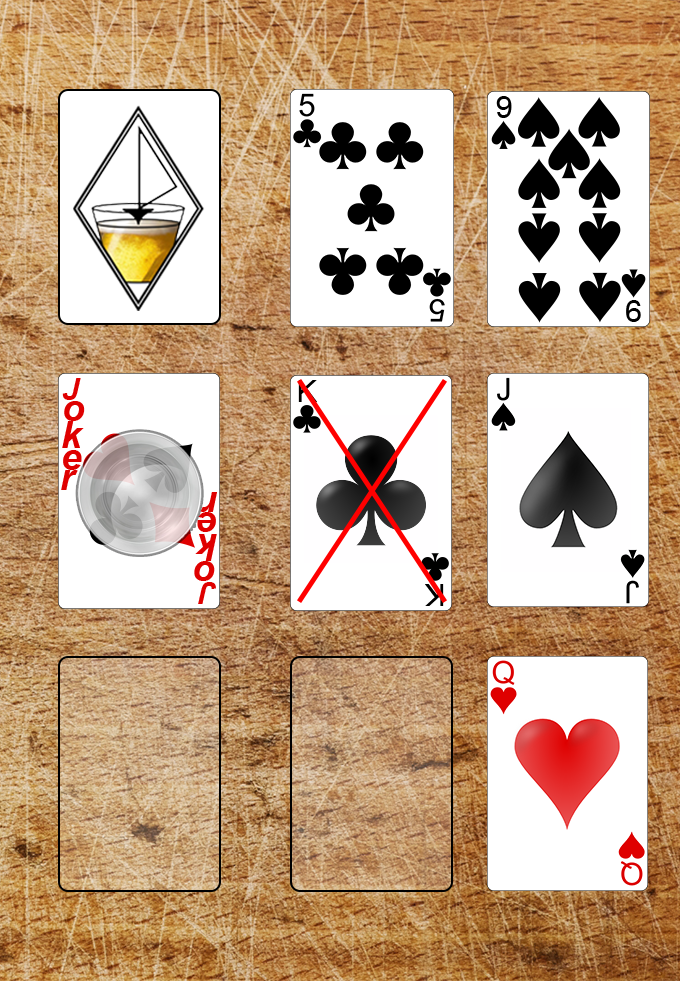
\includegraphics[width=.96\textwidth]{img/cards/Frits_plank_Carolinetje_2.png}
\end{minipage}

\vspace{0.5cm}

\centerline{\Large{\textbf{De rest van dit document bevat de volledige spelregels}}}